%! Author = tomas
%! Date = 9/25/24

% Preamble
\documentclass[11pt, a4paper]{article}
\title{Satelit}
\author{Tomáš Hůla}
\date{Září 2024}

% Packages
\usepackage{amsmath}
\usepackage{tikz}
\usepackage{xcolor}
\usepackage[figurename=Obr.]{caption}
\usepackage{amsfonts}
\usepackage[normalem]{ulem}
\usetikzlibrary{calc}

% Global color definitions
\colorlet{lightgray}{gray!30}
\colorlet{highlight}{blue!50}

% Document
\begin{document}
    \maketitle

    Jelikož se satelit odráží od krajů obdelníku pod stejným úhlem, pod kterým dopadl, má stejné vlastnosti jako paprsky světla odrážející se v zrcadle.
    Základní pravidlo se kterým budeme pracovat je, že zrcadlo znázorňuje objekt, jakoby byl ve stejné vzdálenosti za zrcadlem, jako je objekt od zrcadla.
    Chceme-li paprskem zasáhnout nějaký cíl odrazem o zrcadlo, můžeme paprsek namířit na odraz cíle.
    Paprsek se odrazí od zrcadla ve směru cíle.
    Nutno podotknout, že délka paprsku je stejná jako vzdálenost zdroje od zrcadleného cíle, jelikož paprsek pomyslně cestuje stále rovně do zrcadlené "dimenze".

    \begin{figure}[h]
        \centering
        \begin{tikzpicture}
            % coordinates
            \coordinate (source) at (3, 1);
            \coordinate (target) at (7, 1);
            \coordinate (target-mirrored) at (7, 5);
            \coordinate (mirror-contact) at (5, 3);
            % mirror
            \draw[thick] (0, 3) -- (10, 3);
            % source
            \fill (source) circle (2pt);
            \node[below] at (source) {Zdroj};
            % target
            \draw (target) ++(-0.1,0) -- ++(0.2,0); % Horizontal target line
            \draw (target) ++(0,-0.1) -- ++(0,0.2); % Vertical target line
            \node[below] at (target) {Cíl};
            % target-mirrored
            \draw[lightgray, thick] (target-mirrored) ++(-0.1,0) -- ++(0.2,0); % Horizontal target
            \draw[lightgray, thick] (target-mirrored) ++(0,-0.1) -- ++(0,0.2); % Vertical target
            \node[above] at (target-mirrored) {Odraz cíle};
            % line source -> target-mirroreded
            \draw[thick] (source) -- (mirror-contact);
            % line source -> target-mirroreded
            \draw[lightgray, thick] (mirror-contact) -- (target-mirrored);
            % line intersection -> target
            \draw[thick] (mirror-contact) -- (target);
        \end{tikzpicture}
        \caption{Zrcadlení paprsku}
        \label{fig:mirroring1}
    \end{figure}

    S tímto se dá pracovat i dále, kdy můžeme zrcadlit i zrcadlo.
    Na obrázku \ref{fig:mirroring2} můžeme vidět stejný případ, ale se dvěma zrcadly.

    \begin{figure}[h]
        \centering
        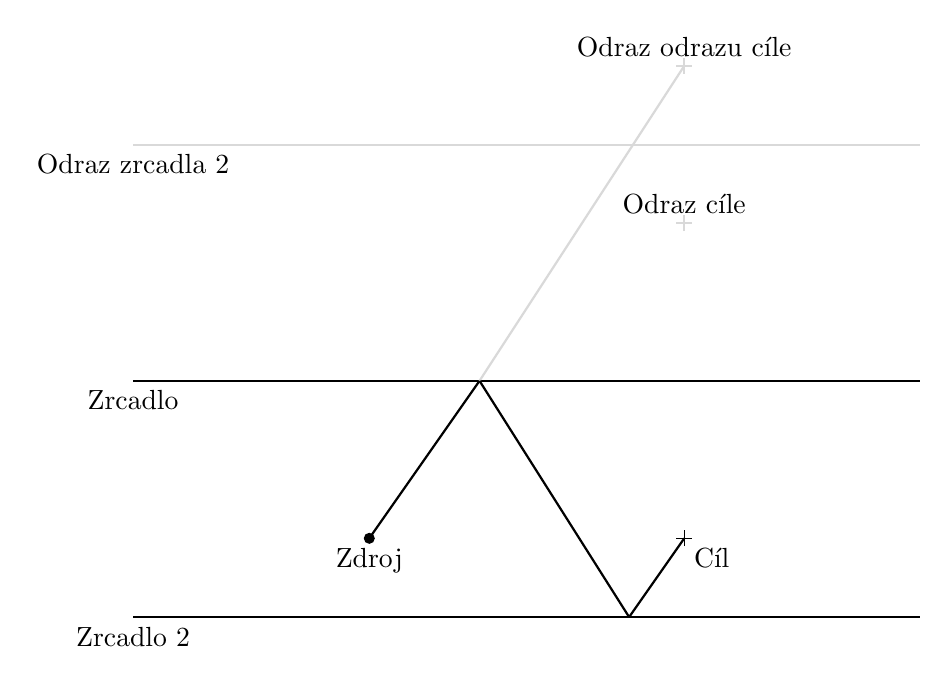
\begin{tikzpicture}
            % coordinates
            \coordinate (source) at (3, 1);
            \coordinate (target) at (7, 1);
            \coordinate (target-mirrored) at (7, 5);
            \coordinate (target-mirrored2) at (7, 7);
            \coordinate (mirror-contact) at (4.4, 3);
            \coordinate (mirror2-contact) at (6.3, 0);
            % first mirror
            \draw[thick] (0, 3) -- (10, 3);
            \node[below] at (0, 3) {Zrcadlo};
            % second mirror
            \draw[thick] (0, 0) -- (10, 0);
            \node[below] at (0, 0) {Zrcadlo 2};
            % second mirror reflection
            \draw[lightgray, thick] (0, 6) -- (10, 6);
            \node[below] at (0, 6) {Odraz zrcadla 2};
            % source
            \fill (source) circle (2pt);
            \node[below] at (source) {Zdroj};
            % target
            \draw (target) ++(-0.1,0) -- ++(0.2,0); % horizontal cross line
            \draw (target) ++(0,-0.1) -- ++(0,0.2); % vertical cross line
            \node[below right] at (target) {Cíl};
            % target-mirrored
            \draw[lightgray, thick] (target-mirrored) ++(-0.1,0) -- ++(0.2,0); % horizontal cross line
            \draw[lightgray, thick] (target-mirrored) ++(0,-0.1) -- ++(0,0.2); % vertical cross line
            \node[above] at (target-mirrored) {Odraz cíle};
            % target-mirrored2
            \draw[lightgray, thick] (target-mirrored2) ++(-0.1,0) -- ++(0.2,0); % horizontal cross line
            \draw[lightgray, thick] (target-mirrored2) ++(0,-0.1) -- ++(0,0.2); % vertical cross line
            \node[above] at (target-mirrored2) {Odraz odrazu cíle};
            % line source -> intersect1
            \draw[thick] (source) -- (mirror-contact);
            % line mirror-contact -> target-mirrored2
            \draw[lightgray, thick] (mirror-contact) -- (target-mirrored2);
            % line mirror-contact -> mirror2-contact
            \draw[thick] (mirror-contact) -- (mirror2-contact);
            % line mirror2-contact -> target
            \draw[thick] (mirror2-contact) -- (target);
        \end{tikzpicture}
        \caption{Zrcadlení paprsku s více zrcadly}
        \label{fig:mirroring2}
    \end{figure}

    V našem případě je zdroj satelit, paprsek jeho trajektorie, zrcadla jsou strany obdelníku a cíle jsou jeho 4 rohy.

    \begin{figure}[h]
        \center
        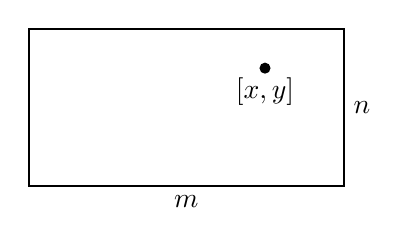
\begin{tikzpicture}
            % coordinates
            \coordinate (satellite) at (3, 1.5);
            % rectangle
            \draw[thick] (0, 0) rectangle (4,2);
            % side labels
            \node[below] at (2, 0) {$m$};
            \node[right] at (4, 1) {$n$};
            % satellite
            \fill (satellite) circle (2pt);
            % satellite label
            \node[below] at (satellite) {$[x,y]$};
        \end{tikzpicture}
        \caption{Satelit v obdelníku}
        \label{fig:satellite}
    \end{figure}

    Když nyní zakreslíme \emph{nekonečně} mnoho odrazů stran obdelníku a tím pádem i jejich rohů, dostaneme obrázek \ref{fig:satellite-mirrors}.
    (odrazy satelitu nezakreslujeme, jelikož to nemá význam pro řešení problému; každý roh je znázorněn křížkem)

    \begin{figure}[h]
        \centering
        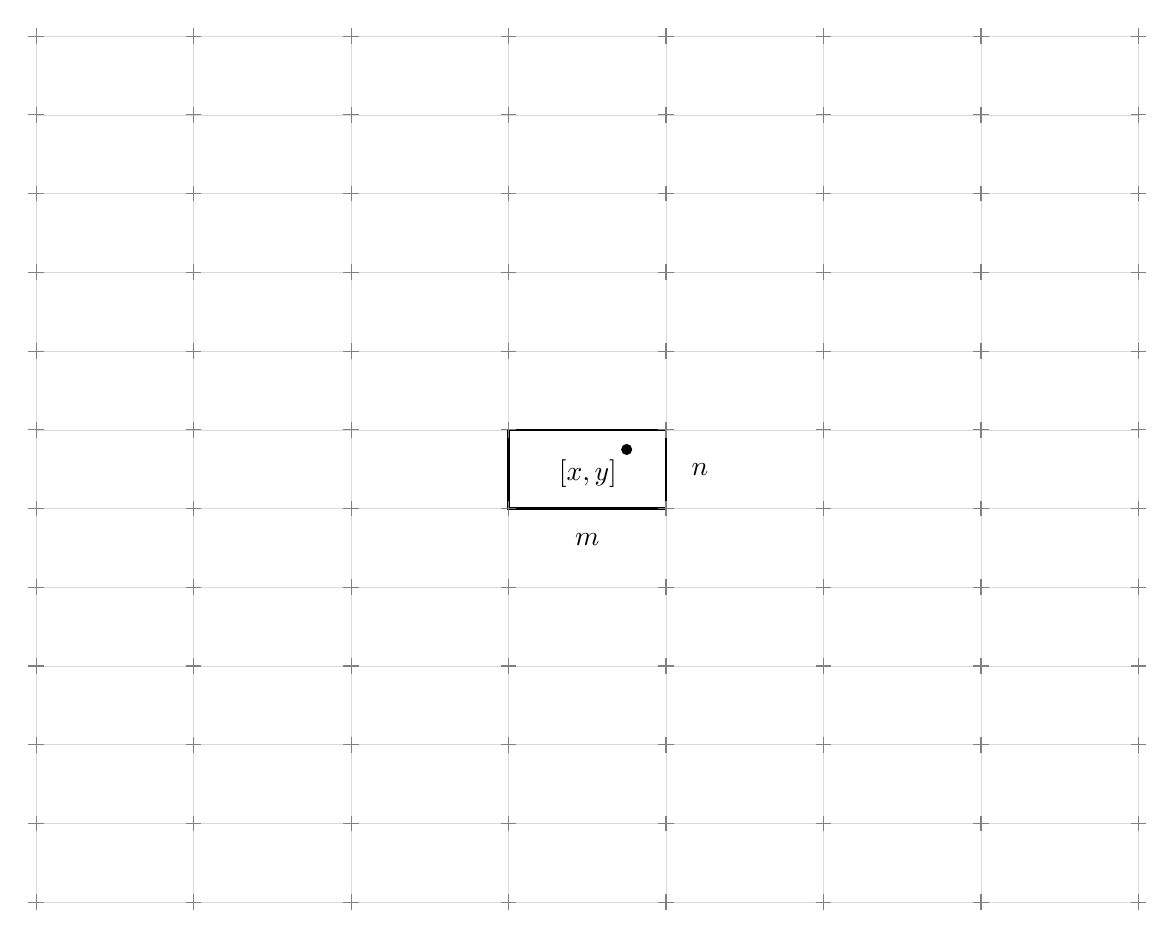
\begin{tikzpicture}
            % coordinates
            \coordinate (rect) at (6,5); % rect bottom-left
            \coordinate (satellite) at ($(rect) + (1.5, 0.75)$);
            % grid
            \draw[lightgray,very thin] (0,0) grid[xstep=2cm,ystep=1cm] (14,11);
            % rectangle
            \draw[thick] (rect) rectangle ++(2,1);
            % side labels
            \node[below] at ($(rect) + (1, -0.2)$) {$m$};
            \node[right] at ($(rect) + (2.2, 0.5)$) {$n$};
            % satellite
            \fill (satellite) circle (2pt);
            % satellite label
            \node[below left] at (satellite) {$[x, y]$};
            % crosses (+) at grid intersections
            \foreach \x in {0,2,...,14} {
                \foreach \y in {0,1,...,11} {
                    \draw[gray] (\x,\y) ++(-0.1,0) -- ++(0.2,0); % horizontal cross line
                    \draw[gray] (\x,\y) ++(0,-0.1) -- ++(0,0.2); % vertical cross line
                }
            }
        \end{tikzpicture}
        \caption{Satelit v obdelníku zrcadlený}
        \label{fig:satellite-mirrors}
    \end{figure}

    Takto vidíme všechny zrcadlové zobrazení rohů obdelníku.


    \section{Otázka 1}
    \label{sec:otazka-1}

    Délka odrážející se trajektorie z počátku satelitu končící v rohu se dá spočítat vzdáleností počátku satelitu k zrcadlovému vyzobrazení daného rohu.

    \textbf{Všechny zobrazení rohu, jež jsou ve vzdálenosti $\leq D$ od satelitu, jsou satelitem po několika odrazech dosažitelné.}
    Toto je znázorněno na obrázku \ref{fig:satellite-radius}.

    \begin{figure}[h]
        \centering
        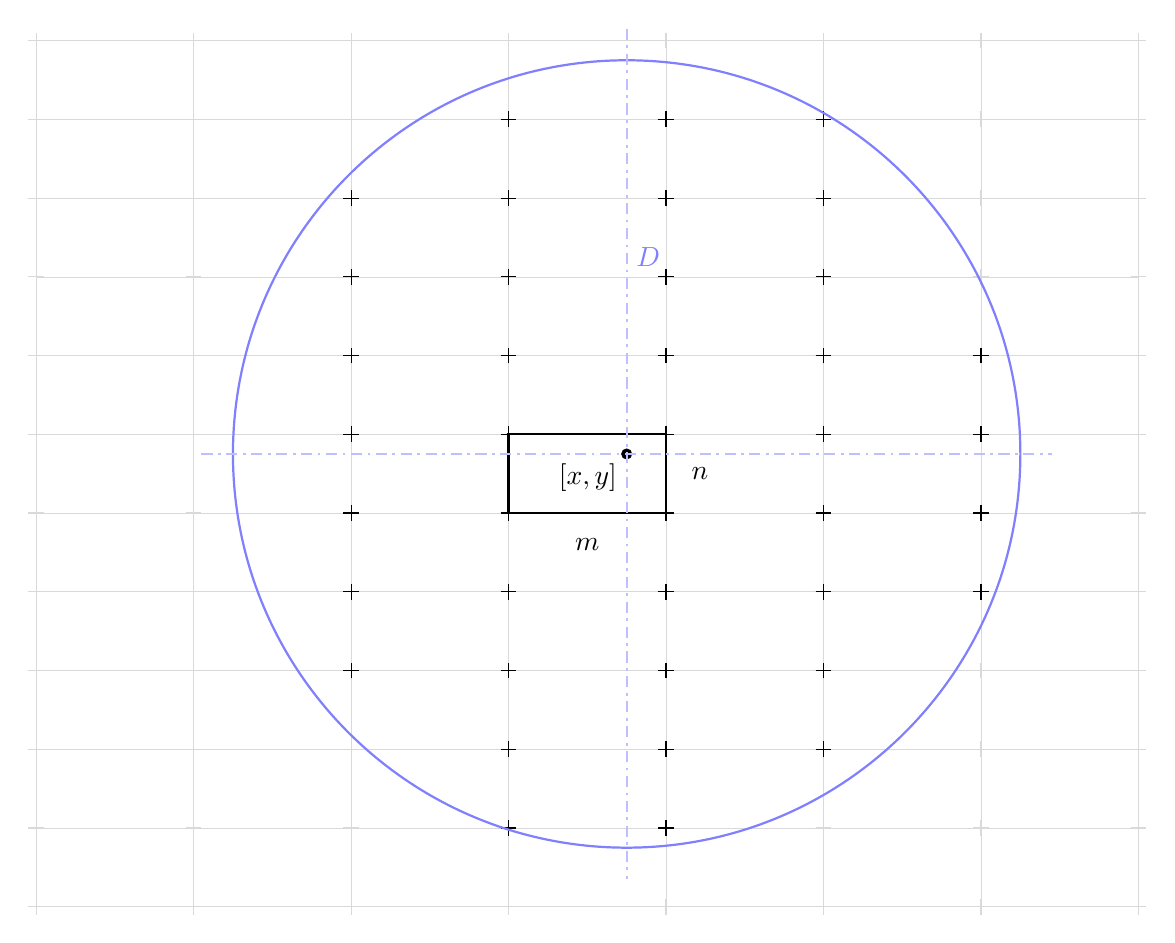
\begin{tikzpicture}
            % coordinates
            \coordinate (rect) at (6,5); % rect bottom-left
            \coordinate (satellite) at ($(rect) + (1.5, 0.75)$);
            % grid
            \draw[lightgray,very thin] (0,0) grid[xstep=2cm,ystep=1cm] (14,11);
            % rectangle
            \draw[thick] (rect) rectangle ++(2,1);
            % side labels
            \node[below] at ($(rect) + (1, -0.2)$) {$m$};
            \node[right] at ($(rect) + (2.2, 0.5)$) {$n$};
            % satellite
            \fill (satellite) circle (2pt);
            % satellite label
            \node[below left] at (satellite) {$[x, y]$};

            % crosses (+) at grid intersections with distance-based color
            \foreach \x in {0,2,...,14} {
                \foreach \y in {0,1,...,11} {
                    % Calculate the distance from satellite to the grid intersection
                    \pgfmathsetmacro{\dx}{\x - (6 + 1.5)}
                    \pgfmathsetmacro{\dy}{\y - (5 + 0.75)}
                    \pgfmathsetmacro{\distance}{sqrt(\dx * \dx + \dy * \dy)}
                    % Check if the distance is less than or equal to 5
                    \pgfmathparse{\distance <= 5 ? 1 : 0}
                    \ifnum
                        \pgfmathresult=1
                        \draw[black] (\x,\y) ++(-0.1,0) -- ++(0.2,0); % horizontal cross line (black)
                        \draw[black] (\x,\y) ++(0,-0.1) -- ++(0,0.2); % vertical cross line (black)
                    \else
                        \draw[lightgray] (\x,\y) ++(-0.1,0) -- ++(0.2,0); % horizontal cross line (gray)
                        \draw[lightgray] (\x,\y) ++(0,-0.1) -- ++(0,0.2); % vertical cross line (gray)
                    \fi
                }
            }

            % circle at (satellite) radius 5
            \draw[highlight, thick] (satellite) circle (5cm);

            % circle axis
            \draw[highlight!50, thick, dash pattern=on 4pt off 2pt on 1pt off 2pt]
            ($(satellite) + (-5.4, 0)$) -- ($(satellite) + (5.4, 0)$); % Horizontal axis
            \draw[highlight!50, thick, dash pattern=on 4pt off 2pt on 1pt off 2pt]
            ($(satellite) + (0, 5.4)$) -- ($(satellite) + (0, -5.4)$); % Vertical axis

            % Label on the circle
            \node[right, text=highlight] at ($(satellite) + (0, 2.5)$) {$D$};

        \end{tikzpicture}
        \caption{Rohy v dosahu satelitu}
        \label{fig:satellite-radius}
    \end{figure}

    Pokud bychom toto měli vyjádřit matematicky, tak můžeme definovat dvě množiny, které vyjadřují horizontální a vertikální body rohů.
    Množiny jsou omezeny pouze na ta čísla, která jsou do vzdálenosti $D$ od satelitu.
    Ale pozor, pouze do vzdálenosti v dané ose.
    (nikoli skutečné rovinové vzdálenosti)

    \begin{gather*}
        H = \left\{ \mathbf{n} \in \mathbb{Z} \mid \mathbf{n} \in \left\langle \frac{-D+x}{m}; \frac{D+x}{m} \right\rangle \right\}\\
        V = \left\{ \mathbf{n} \in \mathbb{Z} \mid \mathbf{n} \in \left\langle \frac{-D+y}{n}; \frac{D+y}{n} \right\rangle \right\}\\
    \end{gather*}

    Množina $H$ jsou celá čísla z \emph{horizontální osy}, vyjadřující i-tý roh na který satelit \emph{"dosáhne"}.
    Množina $V$ jsou celá čísla z \emph{vertikální osy}, vyjadřující i-tý roh na která satelit \emph{"dosáhne"}.
    Nyní $H \times V$ jsou polohy (v rámci pomyslné mřížky, nikoliv souřadnicového systému) všech rohů, do kterých \sout{satelit může doletět}.
    Není to pravda, $H \times V$ jsou všechny rohy v pomyslném čtverci o stranách $D$, nikoli kruhu.
    Takže chceme-li dostat všechny rohy, do kterých satelit může doletět, vyjádříme je takto množino $R$.

    \[
        R = \left| \{ [h, v] \in H \times V \mid \sqrt{(mh - x)^2+(nv - y)^2} \leq D \} \right|
    \]

    Toto je náš výsledek.
    \textbf{Satelit se může rozletět $|R|$ směry, tak, že po nějaké vzdálenosti $d \leq D$ skončí v rohu.}


    \section{Otázka 2}

    Druhá otázka je velmi podobná té první, akorát místo maximální vzdálenosti $D$ máme zadán maximální počet odrazů $N$.
    Definujme si pomocnou funkci $f(x)$, která od kladných čísel odečítá $1$.

    \[
        f(x) = \begin{cases}
                   x - 1 & \text{pro } x > 0 \\
                   x & \text{pro ostatní}
        \end{cases}
    \]

    Nyní si opět definujeme množiny horizontálních a vertikálních bodů mřížky s rohy.
    K $N$ se přičítá $1$, protože první roh je dosažitelný bez odrazu.

    \begin{gather*}
        H = \left\{ \mathbf{n} \in \mathbb{Z} \mid \mathbf{n} \in \left\langle -N; N+1 \right\rangle \right\}\\
        V = \left\{ \mathbf{n} \in \mathbb{Z} \mid \mathbf{n} \in \left\langle -N; N+1 \right\rangle \right\}\\
    \end{gather*}

    Výsledna množina všech dosažitelných rohů by vypadala takto:

    \[
        R = \left| \{ [h, v] \in H \times V \mid |f(v)| + |f(h)| \leq N \} \right|
    \]

    Toto je náš výsledek.
    \textbf{Satelit se může rozletět $|R|$ směry, tak, že po $n \leq N$ odrazech skončí v rohu.}

\end{document}
